\documentclass{standalone}
\usepackage{tikz}
\usetikzlibrary{patterns, positioning}


\begin{document}
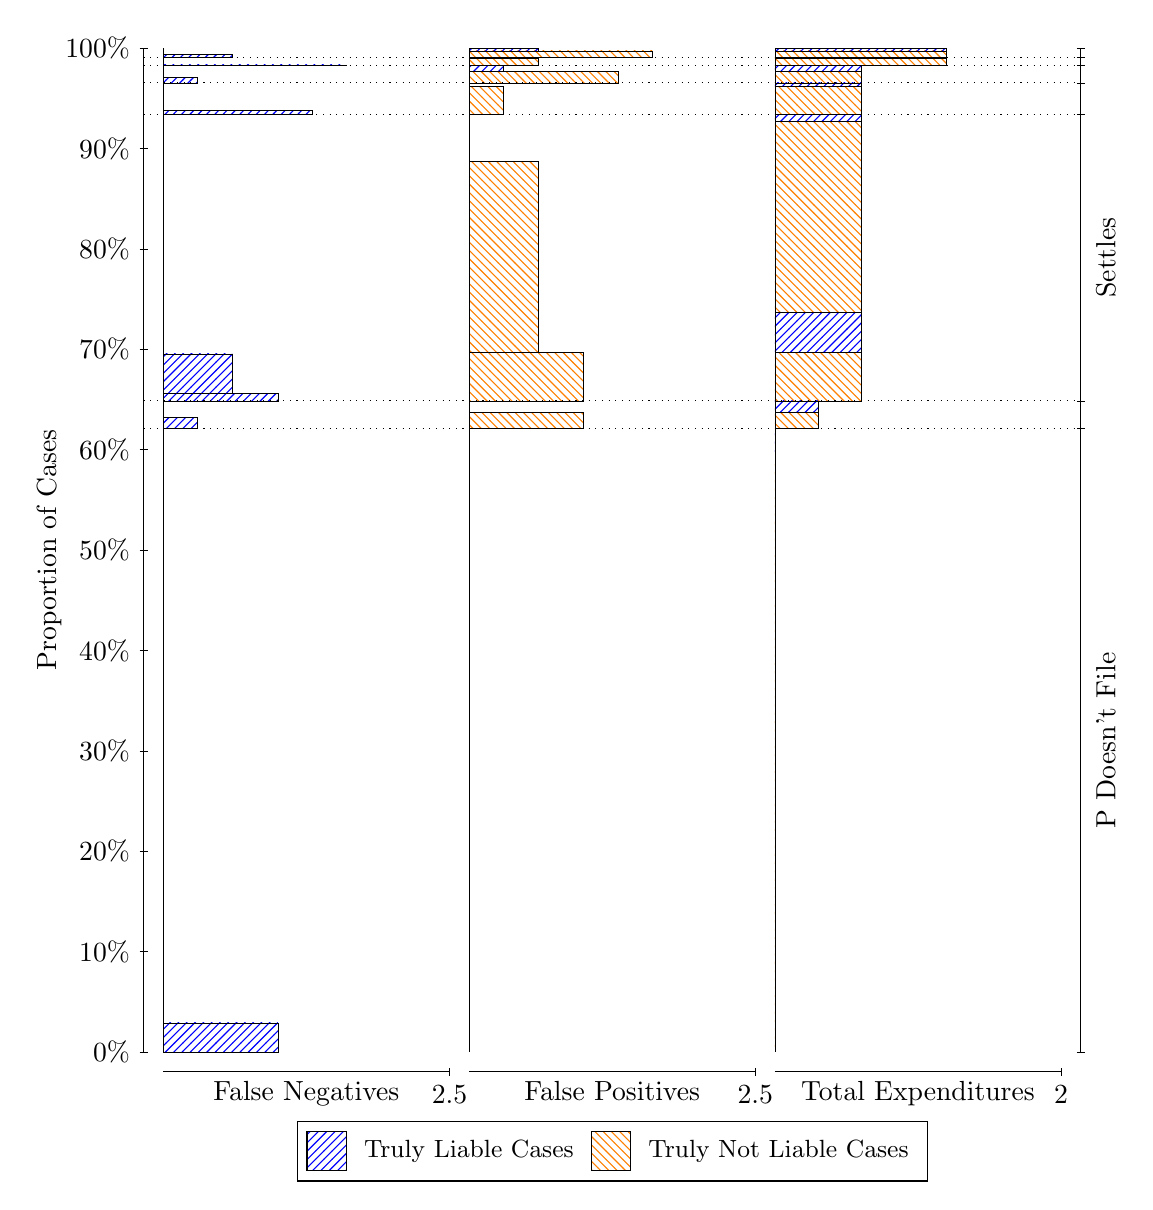
\begin{tikzpicture}
\draw[black, very thin] (1.5,1.75) -- (1.5,14.5);
\node[rotate=90, text=black, anchor=center] at (0.3, 8.125) {Proportion of Cases};
\draw[black, very thin] (1.45,1.75) -- (1.55,1.75);
\node[text=black, anchor=east] at (1.45, 1.75) {0\%};
\draw[black, very thin] (1.45,3.025) -- (1.55,3.025);
\node[text=black, anchor=east] at (1.45, 3.025) {10\%};
\draw[black, very thin] (1.45,4.3) -- (1.55,4.3);
\node[text=black, anchor=east] at (1.45, 4.3) {20\%};
\draw[black, very thin] (1.45,5.575) -- (1.55,5.575);
\node[text=black, anchor=east] at (1.45, 5.575) {30\%};
\draw[black, very thin] (1.45,6.85) -- (1.55,6.85);
\node[text=black, anchor=east] at (1.45, 6.85) {40\%};
\draw[black, very thin] (1.45,8.125) -- (1.55,8.125);
\node[text=black, anchor=east] at (1.45, 8.125) {50\%};
\draw[black, very thin] (1.45,9.4) -- (1.55,9.4);
\node[text=black, anchor=east] at (1.45, 9.4) {60\%};
\draw[black, very thin] (1.45,10.675) -- (1.55,10.675);
\node[text=black, anchor=east] at (1.45, 10.675) {70\%};
\draw[black, very thin] (1.45,11.95) -- (1.55,11.95);
\node[text=black, anchor=east] at (1.45, 11.95) {80\%};
\draw[black, very thin] (1.45,13.225) -- (1.55,13.225);
\node[text=black, anchor=east] at (1.45, 13.225) {90\%};
\draw[black, very thin] (1.45,14.5) -- (1.55,14.5);
\node[text=black, anchor=east] at (1.45, 14.5) {100\%};

\draw[black, very thin] (13.4,1.75) -- (13.4,14.5);
\draw[black, very thin] (13.35,1.75) -- (13.45,1.75);
\node[anchor=west] at (13.35, 1.75) {};
\draw[black, very thin] (13.35,9.6656) -- (13.45,9.6656);
\node[anchor=west] at (13.35, 9.6656) {};
\draw[black, very thin] (13.35,10.02) -- (13.45,10.02);
\node[anchor=west] at (13.35, 10.02) {};
\draw[black, very thin] (13.35,13.66) -- (13.45,13.66);
\node[anchor=west] at (13.35, 13.66) {};
\draw[black, very thin] (13.35,14.057) -- (13.45,14.057);
\node[anchor=west] at (13.35, 14.057) {};
\draw[black, very thin] (13.35,14.276) -- (13.45,14.276);
\node[anchor=west] at (13.35, 14.276) {};
\draw[black, very thin] (13.35,14.38) -- (13.45,14.38);
\node[anchor=west] at (13.35, 14.38) {};
\draw[black, very thin] (13.35,14.5) -- (13.45,14.5);
\node[anchor=west] at (13.35, 14.5) {};

\draw[black, very thin, pattern color=blue, pattern=north east lines] (1.75,1.75) rectangle (3.2033,2.1198);
\draw[black, very thin, pattern color=orange, pattern=north west lines] (1.75,2.1198) rectangle (1.75,9.6656);
\draw[black, very thin, pattern color=blue, pattern=north east lines] (1.75,9.6656) rectangle (2.186,9.8085);
\draw[black, very thin, pattern color=orange, pattern=north west lines] (1.75,9.8085) rectangle (1.75,10.02);
\draw[black, very thin, pattern color=blue, pattern=north east lines] (1.75,10.02) rectangle (3.2033,10.114);
\draw[black, very thin, pattern color=blue, pattern=north east lines] (1.75,10.114) rectangle (2.622,10.616);
\draw[black, very thin, pattern color=orange, pattern=north west lines] (1.75,10.616) rectangle (1.75,13.66);
\draw[black, very thin, pattern color=blue, pattern=north east lines] (1.75,13.66) rectangle (3.6393,13.709);
\draw[black, very thin, pattern color=orange, pattern=north west lines] (1.75,13.709) rectangle (1.75,14.057);
\draw[black, very thin, pattern color=blue, pattern=north east lines] (1.75,14.057) rectangle (2.186,14.13);
\draw[black, very thin, pattern color=orange, pattern=north west lines] (1.75,14.13) rectangle (1.75,14.276);
\draw[black, very thin, pattern color=blue, pattern=north east lines] (1.75,14.276) rectangle (4.0753,14.285);
\draw[black, very thin, pattern color=orange, pattern=north west lines] (1.75,14.285) rectangle (1.75,14.38);
\draw[black, very thin, pattern color=blue, pattern=north east lines] (1.75,14.38) rectangle (2.622,14.415);
\draw[black, very thin, pattern color=orange, pattern=north west lines] (1.75,14.415) rectangle (1.75,14.5);
\draw[black, very thin, pattern color=orange, pattern=north west lines] (5.6333,1.75) rectangle (5.6333,9.2958);
\draw[black, very thin, pattern color=blue, pattern=north east lines] (5.6333,9.2958) rectangle (5.6333,9.6656);
\draw[black, very thin, pattern color=orange, pattern=north west lines] (5.6333,9.6656) rectangle (7.0867,9.8773);
\draw[black, very thin, pattern color=blue, pattern=north east lines] (5.6333,9.8773) rectangle (5.6333,10.02);
\draw[black, very thin, pattern color=orange, pattern=north west lines] (5.6333,10.02) rectangle (7.0867,10.637);
\draw[black, very thin, pattern color=orange, pattern=north west lines] (5.6333,10.637) rectangle (6.5053,13.064);
\draw[black, very thin, pattern color=blue, pattern=north east lines] (5.6333,13.064) rectangle (5.6333,13.66);
\draw[black, very thin, pattern color=orange, pattern=north west lines] (5.6333,13.66) rectangle (6.0693,14.008);
\draw[black, very thin, pattern color=blue, pattern=north east lines] (5.6333,14.008) rectangle (5.6333,14.057);
\draw[black, very thin, pattern color=orange, pattern=north west lines] (5.6333,14.057) rectangle (7.5227,14.204);
\draw[black, very thin, pattern color=blue, pattern=north east lines] (5.6333,14.204) rectangle (6.0693,14.276);
\draw[black, very thin, pattern color=orange, pattern=north west lines] (5.6333,14.276) rectangle (6.5053,14.37);
\draw[black, very thin, pattern color=blue, pattern=north east lines] (5.6333,14.37) rectangle (5.6333,14.38);
\draw[black, very thin, pattern color=orange, pattern=north west lines] (5.6333,14.38) rectangle (7.9587,14.465);
\draw[black, very thin, pattern color=blue, pattern=north east lines] (5.6333,14.465) rectangle (6.5053,14.5);
\draw[black, very thin, pattern color=orange, pattern=north west lines] (9.5167,1.75) rectangle (9.5167,9.2958);
\draw[black, very thin, pattern color=blue, pattern=north east lines] (9.5167,9.2958) rectangle (9.5167,9.6656);
\draw[black, very thin, pattern color=orange, pattern=north west lines] (9.5167,9.6656) rectangle (10.062,9.8773);
\draw[black, very thin, pattern color=blue, pattern=north east lines] (9.5167,9.8773) rectangle (10.062,10.02);
\draw[black, very thin, pattern color=orange, pattern=north west lines] (9.5167,10.02) rectangle (10.607,10.637);
\draw[black, very thin, pattern color=blue, pattern=north east lines] (9.5167,10.637) rectangle (10.607,11.139);
\draw[black, very thin, pattern color=orange, pattern=north west lines] (9.5167,11.139) rectangle (10.607,13.566);
\draw[black, very thin, pattern color=blue, pattern=north east lines] (9.5167,13.566) rectangle (10.607,13.66);
\draw[black, very thin, pattern color=orange, pattern=north west lines] (9.5167,13.66) rectangle (10.607,14.008);
\draw[black, very thin, pattern color=blue, pattern=north east lines] (9.5167,14.008) rectangle (10.607,14.057);
\draw[black, very thin, pattern color=orange, pattern=north west lines] (9.5167,14.057) rectangle (10.607,14.204);
\draw[black, very thin, pattern color=blue, pattern=north east lines] (9.5167,14.204) rectangle (10.607,14.276);
\draw[black, very thin, pattern color=orange, pattern=north west lines] (9.5167,14.276) rectangle (11.697,14.37);
\draw[black, very thin, pattern color=blue, pattern=north east lines] (9.5167,14.37) rectangle (11.697,14.38);
\draw[black, very thin, pattern color=orange, pattern=north west lines] (9.5167,14.38) rectangle (11.697,14.465);
\draw[black, very thin, pattern color=blue, pattern=north east lines] (9.5167,14.465) rectangle (11.697,14.5);
\draw[black, dotted] (1.5,9.6656) -- (13.4,9.6656);
\draw[black, dotted] (1.5,10.02) -- (13.4,10.02);
\draw[black, dotted] (1.5,13.66) -- (13.4,13.66);
\draw[black, dotted] (1.5,14.057) -- (13.4,14.057);
\draw[black, dotted] (1.5,14.276) -- (13.4,14.276);
\draw[black, dotted] (1.5,14.38) -- (13.4,14.38);
\draw[black, very thin] (1.75,1.5) -- (5.3833,1.5);
\node[text=black, anchor=north] at (3.5667, 1.5) {False Negatives};
\draw[black, very thin] (5.3833,1.45) -- (5.3833,1.55);
\node[text=black, anchor=north] at (5.3833, 1.45) {2.5};

\draw[black, very thin] (5.6333,1.5) -- (9.2667,1.5);
\node[text=black, anchor=north] at (7.45, 1.5) {False Positives};
\draw[black, very thin] (9.2667,1.45) -- (9.2667,1.55);
\node[text=black, anchor=north] at (9.2667, 1.45) {2.5};

\draw[black, very thin] (9.5167,1.5) -- (13.15,1.5);
\node[text=black, anchor=north] at (11.333, 1.5) {Total Expenditures};
\draw[black, very thin] (13.15,1.45) -- (13.15,1.55);
\node[text=black, anchor=north] at (13.15, 1.45) {2};

\node[text=black, centered, rotate=90] at (13.72, 5.7078) {P Doesn't File};

\node[text=black, centered, rotate=90] at (13.72, 11.84) {Settles};





\draw (7.449999999999999,1.5) node[draw=none] (baseCoordinate) {};
\begin{scope}[align=center]
        \matrix[scale=0.5, draw=black, below=0.5cm of baseCoordinate, nodes={draw}, column sep=0.1cm]{
            \node[rectangle, draw, minimum width=0.5cm, minimum height=0.5cm, pattern color=blue, pattern=north east lines] {}; &
            \node[draw=none, font=\small, text=black] (B) {Truly Liable Cases}; &
            \node[rectangle, draw, minimum width=0.5cm, minimum height=0.5cm, pattern color=orange, pattern=north west lines] {}; &
            \node[draw=none, font=\small, text=black] (B) {Truly Not Liable Cases}; \\
            };
\end{scope}

\end{tikzpicture}
\end{document}